
%%%%%%%%

\chapter{Specification of options \protect\\ 
\eee \eee and IO functions}
\label{chp:spe-opt-io}



The list of possible \emph{options} of a \tafkit command is obtained 
with the (classical) \samp{--help} option.
They fall in the following categories:
\begin{enumerate}
	\item  options that give information on the instance;

	\item  specifications of the alphabet(s);

	\item  determination of the input and output formats;

	\item  activation of benchmarking options;
	
	\item  and finally parametrization of the grammars for rational 
	(\ie regular) expressions.
\end{enumerate}
The description of the options of the first four categories is given 
in the next section;
the one of options controlling the rational expressions, called 
\emph{writing data}, is postponed to the following section.

\section{Simple options}
\label{sec:opt-spe}

Along the Unix tradition, the options are given long names, called 
with the prefix \samp{--}, together with short equivalent names, 
prefixed with a simple \samp{-}, which, in practice, will often be 
prefered.

\subsection{Information options}
\label{ssc:inf-opt}

They are listed in \tabla{inf-opt}.
% The full list of options in a given instance of \tafkit can be obtained with 
% \kbd{vcsn-xx-y --help}.
% \begin{shell}
% $ \kbd{vcsn-char-b --help}
% Usage: vcsn-char-b [OPTION...] <command> <args...>
% VCSN TAF-Kit -- a toolkit for working with automata

% We describe here how the alphabet(s) of an automaton or of an 
% expression, and the input and output formats of a command are 
% specified, that is, how the items~1 and~2 in \sbsct{com-opt} are 
% dealt with.
% The description of the so-called \emph{writing data} is postponed to 
% the next section.

\begin{table}[ht]
\begin{center}
\begin{tabular}{>{\ttfamily}l>{\ttfamily\e}lp{.7\textwidth}}
\hline
\multicolumn{1}{c}{long option} & 
\multicolumn{1}{c}{short} & 
\multicolumn{1}{c}{purpose of the option} \\
  \hline
  \Option{help}  &  \ShortOpt{?}\e &             Give the help list\\
  \Option{usage} &   &         Give a short usage message \\
  \Option{version} &  \ShortOpt{V} &        Print program version \\
 \Option{list-commands} &  \ShortOpt{l}  &   List usual commands\\
 \Option{list-all-commands} & \ShortOpt{L} &   List all commands, including debug 
 commands\\
 \Option{list-automata} &  &      List predefined automata \\
%  \Option{list-factory} &  &      List automata factories\\
  \hline
\hline
\end{tabular}
\end{center}
\caption{Information options}
\label{tab:inf-opt}
\end{table}

\Cave 
The character \samp{?} being interpreted by the shell, it should be 
protected in order to be given as an argument to a command.
Without such a protection, the behaviour may depend on the shell, and 
according to the files within the directory.

This option \samp{?} should probably be suppressed, but it is 
necessary for the library \samp{argp} which is used for reading the 
options in the command line and it does not seem easy to get around it.
In any case, it should be avoided, and the \samp{--help} option be 
used. 


\subsection{Alphabet specification}
\label{ssc:alp-spe}


\paragraph{The necessity of alphabet specification}

As we have seen (\sbsct{taf-ins}), every \tafkit instance determines 
(or one could say, is determined by) the type of the letters that 
generate the free monoid(s) over which the automata or the rational 
expressions are built.
And this is sufficient at compile time, \ie in order to generate 
\tafkit.

But \vcsn and the \tafkit functions are designed in such a way that 
they need to know the \emph{complete} type of an automaton or an 
expression in order to handle it, \ie not only the type of weights 
and of letters, but also the \emph{set of letters} that constitute the 
alphabet(s).

The \xml files which describe automata, or expressions, contain this 
information and are so to say self-contained.
For instance, when we read
\file{a1.xml} in \secti{fir-con} and determinized this
automaton, we did not have to tell \tafkit that the alphabet was
$A=\{a,b\}$.  
% and already contains this information.
% When a \tafkit instance reads a parameter given as an \xml file, 
% there is no need to specify any other 
% information besides the name of the file.  
On the contrary, when the automaton, or the expression, does not exist 
prior to the \tafkit function, then specifying an alphabet 
\emph{is mandatory}.
For instance, the following commands\footnote{%
   The function \FctInd{edit} is described at \sbsct{io-edi}, 
   \FctInd{exp-to-aut} which takes a rational expression and 
   converts it into an automaton at \sbsct{exp-to-aut}.}
end in error:

\begin{shell}
$ \kbd{vcsn-char-b edit aut.xml}
Error: alphabet should be explicitly defined using --alphabet
$
$ \kbd{vcsn-char-b exp-to-aut 'aba+a'}
Error: alphabet should be explicitly defined using --alphabet
\end{shell}%$

In the latter case moreover, and as there is no \apriori restriction 
on the characters that can be used as letters, \vcsn needs to know the 
alphabet over which the expression is built in order to parse the 
rational expression:
there is no other way for guessing whether the alphabet is 
$A=\{a,b\}$ (and the \samp{+} is a rational operator)
or if the alphabet is $B=\{a,b,+\}$ and the \samp{+} is just a letter.


Specifying the alphabet can be done by
using \option{--alphabet=ab} or its short equivalent \option{-aab}.
For instance, the correct writing of the above command reads:

\begin{shell}
$ \kbd{vcsn-char-b --alphabet=ab edit aut.xml}
...
$ \kbd{vcsn-char-b -aab exp-to-aut 'aba+a' > aut.xml}
$ \kbd{vcsn-char-b display aut.xml}
\end{shell}

\begin{figure}[ht]
    \centering
\includegraphics[scale=0.4]{figures/aut.ps}
\caption{Result of the command \code{vcsn-char-b display aut.xml}}
\end{figure}

\tabla{alp-opt} reviews the alphabet specification options.
The different possibilities: \emph{characters}, \emph{integers}, and 
\emph{pairs} need to be described with more details.

\begin{table}[ht]
\begin{center}
\begin{tabular}{>{\ttfamily}l>{\ttfamily\e}lp{.7\textwidth}}
\hline
\multicolumn{1}{c}{long option} & 
\multicolumn{1}{c}{short} & 
\multicolumn{1}{c}{purpose of the option} \\
  \hline
\Option{alphabet}    & \ShortOpt{a}\e 
     & specify the alphabet of automata or rational expressions 
    \\ %  & \ref{sec:--alphabet}
 \Option{alphabet1}     & \ShortOpt{a}
     & specify the first (or input) alphabet of transducers 
	 (\code{fmp})
    \\ % & \ref{sec:--alphabet}
\Option{alphabet2}    & \ShortOpt{A}
     & specify the second (or output) alphabet of transducers (\code{fmp})
     \\ %& \ref{sec:--alphabet}
%   \samp{--parser} & \samp{-p} & fine-tune the symbols used for input and output of rational expressions and automata & \ref{sec:writingdata}\\
\hline
\end{tabular}
\end{center}
\caption{Alphabet options}
\label{tab:alp-opt}
\end{table}

\paragraph{Character alphabets}

For characters alphabets (as with the \samp{char} \tafkit instances
used in the above examples), the letters of the alphabets can be
arbitrary ASCII characters, and need just to be listed after
the \samp{--alphabet=} or \samp{-a} option.
Some character alphabets are predefined.  These are:

\begin{center}
\begin{tabular}{lll}
\samp{letters} & for & the lower case letters $\{a,b,\ldots,z\}$.\\
\samp{alpha} & for & the upper and lower case letters $\{a,b,\ldots,z,A,B,\ldots,Z\}$.\\
\samp{digits} & for & all digits $\{0,1,\ldots,9\}$.\\
% \samp{ascii} & All ASCII characters.\\
\end{tabular}
\end{center}

\noindent
For instance, \samp{-aletters} is an abbreviation for
\samp{-aabcdefghijklmnopqrstuvwxyz}.  
The above list of \emphind{predefined alphabets} is obtained by typing \samp{vcsn-char-b --help}.

When specifying characters alphabets, the following characters have 
to be escaped with a backslash: 

\medskipneg \medskipneg 
\begin{center}
\PushLine
\verb*| | (space)
\PushLine 
\samp{'}
\PushLine 
\samp{"}
\PushLine 
\samp{(}
\PushLine 
\samp{)}
\PushLine 
\samp{=}
\PushLine 
\samp{,}
\PushLine 
\samp{\bslash}
\PushLine 
\end{center}
and in this case the list of characters has to be put within quotes.
The same characters are then used normally --- without being escaped 
--- in the expression.
For instance, the following
commands will create an automaton that recognize all `decimal' numbers 
written in base~2, and then display the quotient\footnote{%
    The function \FctInd{quotient} is described at 
	\sbsct{aut-mul-quo}; 
	\samp{dec-bin.xml} is an automaton with 12 states and 27 
	transitions and diplaying it would have been messy.}.

\begin{shell}
$ \kbd{vcsn-char-b -a'01\bslash,' exp-to-aut '1(0+1)*+(1(0+1)*+0),(0+1)(0+1)*' > dec-bin.xml}
$ \kbd{vcsn-char-b quotient dec-bin.xml \bslash| display -}
\end{shell}

\begin{figure}[ht]
    \centering
\includegraphics[scale=0.4]{figures/dec-bin.ps}
\caption{Result of the command \code{vcsn-char-b quotient dec-bin.xml \bslash| display -}}
\end{figure}


\paragraph{Integer alphabets}

The letters of an integer alphabet must be specified as signed integer
(they are represented by the \Cpp type \texttt{int}), and should be
separated by commas.  
For instance, the following command will
construct an automaton that reads any sequence of coins of $1$, $2$,
$5$, $10$, $20$, or $50$ cents, as long as the values are increasing.

\begin{shell}
$ \kbd{vcsn-int-b -a1,2,5,10,20,50 exp-to-aut '1*2*5*10*20*50*' > coins.xml}
$ \kbd{vcsn-int-b eval coins.xml '1210'}
1
$ \kbd{vcsn-int-b eval coins.xml '12105'}
0
$ \kbd{vcsn-int-b eval coins.xml '121050'}
1
\end{shell}%$

Note that \emph{digits} are \emph{characters} and not 
\emph{integers}, even if they look like the latter (for integers 
between~0 and~9) and if, in \vcsnv, no operations on integer letters 
are implemented that could differentiate them.
The only difference is thus the syntax when listing them in the 
option. 

\paragraph{Pair alphabets}

Pair alphabets should be specified using parentheses and commas to
form pairs --- with types of letter that match the \tafkit instance, of 
course ---, as in the following example:

\begin{shell}
$ \kbd{vcsn-char-int-b -a'(a,1)(a,-1)(b,2)' exp-to-aut '((a,-1)+(a,1))(b,2)' > misc.xml}
$ \kbd{vcsn-char-int-b display misc.xml}
\end{shell}

\begin{figure}[ht]
    \centering
\includegraphics[scale=0.4]{figures/misc.ps}
\caption{Result of the command \code{vcsn-char-int-b display misc.xml}}
\end{figure}

\paragraph{Alphabets for transducers}

The products of two free monoids have two alphabets, one for each monoid.  
The instances of \tafkit that handle transducers consequently support 
two options \samp{--alphabet1=} and \samp{--alphabet2=}, that can be
abbreviated  to \samp{-a} and \samp{-A} respectively.
\tabla{tfk-ins} gives the two possible choices for these alphabets in 
\tafkitv: both 
\emph{character}, or both \emph{integer}, alphabets.
The following command calls for the interactive construction of the 
right normaliser for numbers written in base~2 which is then shown 
below (\cf \cite{FrouSaka10}).

\begin{shell}
$ \kbd{vcsn-int-fmp-b -a0,1,2 -A0,1 edit norm2.xml}
...
\end{shell}

\begin{figure}[ht]
    \centering
\includegraphics[scale=0.4]{figures/norm2.ps}
\caption{The normaliser in base 2}
\end{figure}

\Cave 
The function \FctInd{exp-to-aut} is not implemented in \tafkitv 
for the \code{fmp} instances (\cf \secti{fmp-fct}).

\paragraph{Unix usage}
The command line is first interpreted by the \code{shell}, which 
makes the characters \samp{.}, \samp{?}, \samp{*}, \samp{'}, 
\etc being given their meaning for the \code{shell}.
In order to give them their meaning in the current alphabet and in 
the writing of rational expressions, they have to be protected by 
\samp{'}, or \samp{"}.

\begin{shell}
$ \kbd{vcsn-char-b -aab cat-E aab}
aab
$ \kbd{vcsn-char-b -aab cat-E aa(b)}
zsh: unknown file attribute
$ \kbd{vcsn-char-b -aab cat-E 'aa(b)'}
aa.b
$ \kbd{vcsn-char-b -aab cat-E aab*}
zsh: no matches found: aab*
$ \kbd{vcsn-char-b -aab cat-E "aab*"}
aab*
\end{shell}%$


The normal unix \code{shell} definition, allocation and utilisation 
of variables may be mixed with the usage of \tafkit command lines.
For instance, the following
command will create an automaton that recognize numbers of the form
\samp{12,456,789}, where a comma must be used as thousand separator:

\begin{shell}
$ \kbd{d="(0+1+2+3+4+5+6+7+8+9)"}
$ \kbd{vcsn-char-b exp-to-aut -a'0123456789\bslash,' "($d+$d$d+$d$d$d)(,$d$d$d)*" > numbers.xml}
$ \kbd{vcsn-char-b eval numbers.xml 1,234,987}
1
$ \kbd{vcsn-char-b eval numbers.xml 1,24,987}
0
\end{shell}%$
Note how the expression must be enclosed with \samp{"} rather than 
with \samp{'} in order to be correctly interpreted.

\begin{shell}
$ \kbd{d="(0+1+2+3+4+5+6+7+8+9)"}
$ \kbd{vcsn-char-b exp-to-aut -a'0123456789\bslash,' '($d+$d$d+$d$d$d)(,$d$d$d)*' > numbers.xml}
Lexer error, unrecognized characters: $d+$d$d+$d$d$d)(,$d$d$d)*
\end{shell}%$



\subsection{Input and output formats}
\label{ssc:io-for}

The \tafkit commands are supposed to input and output objects of 
different sorts: automata,
rational expressions, words, weights and Boolean results.
Their formats are controlled by the attributes of the input and 
output options.
As shown on \tabla{io-for}, there is one default format when no 
format option is called.

\begin{table}[ht]
\begin{center}
\begin{tabular}{>{\ttfamily}l>{\ttfamily\e}lp{.7\textwidth}}
\hline
\multicolumn{1}{c}{long option} & 
\multicolumn{1}{c}{short} & 
\multicolumn{1}{c}{purpose of the option} \\
\hline
\Option{input} & \ShortOpt{i} & 
select input format for automata and rational expressions 
\\ 
\Option{output} & \ShortOpt{o} & 
select output format for automata and rational expressions 
\\ 
\Option{verbose} & \ShortOpt{v}& 
select verbose option for Boolean results 
    \\ 
\hline
\end{tabular}
\end{center}

\medskip
\begin{center}
\begin{tabular}{>{\e}l>{\e}lcc}
    \hline
\multicolumn{1}{c}{\code{-i} values\e} & 
\multicolumn{1}{c}{\code{-o} values\e} & 
\e  format for automata \e & 
\e format for rational expressions \\
  \hline
  (none)     & (none)     & 
  \fsmxml              & text string \\
  \code{xml} & \code{xml} &
  \fsmxml              & \fsmxml \\
  \code{fsm} &  \code{fsm} &  
  `\fst'                 & --- \\
  --- & \code{dot}  &
  \code{dot}   & --- \\
  \code{exp} & \code{exp} &
  ---              & text string \\
  \code{fpexp} & \code{fpexp} &
  ---              & text string \\
  \hline
\end{tabular}
\end{center}
\caption{Input and output options and formats}
\label{tab:io-for}
\end{table}
\IndirInd{xml}{format}%
\IndirInd{exp}{format}%
\IndirInd{fpexp}{format}%
\IndirInd{fsm}{format}%
\IndirInd{dot}{format}%

These options are used not only to control and adequatly adjust the 
format of data handled by \tafkit in order to process them but allow 
also to make \tafkit a translator between different format for a 
given object.


\subsubsection{Automata formats}
\label{ssc:aut-for}

Automata are always \emph{files}; 
they are read from a file whose filename is specified on the command 
line, and the file is output on the standard output (or can be 
diverted to a named file in the Unix way).   

\vcsn can \emph{read} automata in two formats: 
\fsmxml (the default format), or in a textual format, called 
\code{fsm} and which is close to the one used in \fst.  
\Indextt{OpenFST}%
It can \emph{write} automata in these two formats, as well as in the
\samp{dot} format 
that can then be used for graphical output afterwards.

\paragraph{The \code{xml} format} is the default format for input and  
output automata to and from \vcsn.
It is defined by the \fsmxml format whose complete description will 
be given in a forthcoming technical report (\cf also 
\cite{DemaEtAl08}).

\paragraph{The \code{fsm} format} has been defined within the 
AT\&T FSM Library\texttrademark, Finite-State Machine Library 
\cite{AllaEtAl03} and used in the \fst library \cite{AllaEtAl10}.
\Indexsc{OpenFST}%

\begin{shell}
$ \kbd{vcsn-char-b -ofsm cat b1.xml}
0   0   a    0
0   0   b    0
0   1   b    0
1   1   a    0
1   1   b    0
1    0
\end{shell}%
% $ \kbd{vcsn-char-z -ofsm cat b1.xml \bslash| -ifsm eval - 'bab'}
% 2

\Cave 
The \code{fsm} format is not really implemented in \tafkitv.
It has been added in a way which is more a feasibility proof.
There are indeed two reasons for the limitations of the \code{fsm} 
format within \vcsn. 

First, the automata than can be described with the \code{fsm} format 
must meet several conditions: one initial state only, labels are 
letters (or integers that refer to a symbol table).
Second, \vcsn does not code the weights correctly for \fst.
It is thus inadequate to try to use the \code{fsm} format for another 
automata than `letterized' Boolean automata with a unique initial 
state.
The following two examples of commands use the \code{fsm} format for 
$\Z$-automata.
The first one gives a correct answer, as the weights are all equal 
to~``1'';
the second one demonstrates that \vcsn is not even able to read 
correctly the \code{fsm} file it has written.


\begin{shell}
$ \kbd{vcsn-char-z -ofsm cat b1.xml \bslash| -ifsm eval - 'bab'}
2
\end{shell}%

\begin{shell}
$ \kbd{vcsn-char-z -ofsm cat c1.xml}
0	1	1	 0
0	0	0+1	 0
1	1	(\{2\} 0)+(\{2\} 1)	 0
1	 0
$ \kbd{vcsn-char-z -ofsm cat c1.xml | vcsn-char-z -ifsm -ofsm cat -}
0	1	e	 0
0	0	0	 0
1	 0
\end{shell}%


\paragraph{The \code{dot} format} produces
\code{dot} files that can be processed and visualized using the 
\code{GraphViz} package.
\Indextt{Graphviz}%
The first two comand lines below are equivalent to the third one.

\begin{shell}
$ \kbd{vcsn-char-b -odot cat b1.xml > b1.dot}
$ \kbd{dotty b1.dot}
$ \kbd{vcsn-char-b display b1.xml}
\end{shell}%$
\Indextt{dot}%
\Indextt{dotty}%


\subsubsection{Rational expression formats}
\label{ssc:rat-exp-for}

Rational expressions are given either as \emph{character strings} --- default 
format --- or \xml  \emph{files} --- \code{xml} format.

By default, rational expressions are \emph{read} as strings given on 
the \emph{command line}, 
and \emph{output} as strings on the \emph{standard output}.
Both can be diverted in the Unix way, but a \emph{string} written in a file 
cannot be read by \tafkit directly in this file (\cf \sbsct{fct-cat-E}).

\begin{shell}
$ \kbd{vcsn-char-b -aab cat-E '(a+b(a(b)*a)*b)*'}
(a+b.(a.b*.a)*.b)*
$ \kbd{vcsn-char-b -aab cat-E '(a+b(a(b)*a)*b)*' > exp.txt}
$ \kbd{cat exp.txt}
(a+b.(a.b*.a)*.b)*
$ \kbd{vcsn-char-b -aab cat-E exp.txt}
Lexer error, unrecognized characters: exp.txt
$ \kbd{cat exp.txt | vcsn-char-b -aab cat-E - }
(a+b.(a.b*.a)*.b)*
\end{shell}%$

There are indeed \emph{two} string formats for expressions, 
\code{exp} and \code{fpexp}, when they are made explicit.
The first one stands for \emph{expression}, and is the default 
format, the second one for \emph{fully parenthesized expression}.
They have both the same behaviour for the input.
For the output, the \code{exp} format gives an expression with as few 
parentheses as possible, the \code{fpexp} format gives the expression 
with all parentheses made explicit.
\begin{shell}
$ \kbd{vcsn-char-b -oexp -aab cat-E 'a*(b a)'}
a*.b.a
$ \kbd{vcsn-char-b -ofpexp -aab cat-E 'a*(b a)'}
(((a)*.b).a)
\end{shell}%$


Alternatively, rational expressions can be read from an \fsmxml file whose
filename is given on the command line, and output as an \fsmxml 
file as well.
\begin{shell}
$ \kbd{vcsn-char-b -aab -oxml cat-E '(a+b(a(b)*a)*b)*' > exp.xml}
$ \kbd{vcsn-char-b -ixml cat-E exp.xml}
(a+b.(a.b*.a)*.b)*
\end{shell}%$



\subsubsection{Word formats}
\label{ssc:wor-for}

Words are always \emph{strings} of letters, that are read on the 
command line, and written on the standard output.

\Cave
Although \emph{words} are, from a formal point of view, a (simple) 
instance of a rational expression, \tafkitv handles them as objects 
of different and uninterchangeable types (\cf \sbsct{evl-wrd}).
We come back to the subject in the next section.

\longonly{%
\begin{ComVd}{110515}
	The command \Fct{eval} reads a word, and not an expression.
	It does not seem that there exists indeed a command which 
	outputs a `word' (and not an automaton or an expression).
	
	This will be reworked in the framework where there will be two 
	kinds of expressions.
\end{ComVd}%
}%

\subsubsection{Weight formats}
\label{ssc:wei-for}

Weights, that is, elements of the weight semiring, and such as the 
result of the evaluation of a word in an automaton for instance,
are simply output as \emph{strings} on the standard output.
\begin{shell}
$ \kbd{vcsn-char-z eval c1.xml '101101'}
45
\end{shell}%$
The way they are input, as strings as well, as part of a rational 
expression, is described in the next section.

In one case (in two similar cases indeed), weights will be input as 
argument of a function and not as part of a rational expression. They 
will be written as strings as well, which will raise some problem 
(\cf \sbsct{aut-sta-ext-mul}).


\subsubsection{Boolean result formats}
\label{ssc:boo-res-for}


Some \tafkit functions, such as \Indextt{is-empty} which determines 
whether an automaton is empty or not, yield Boolean results.
In the default format, such results are returned using the
\emph{status code} of the \tafkit instance, so that the correponding
commands can be used as conditions in \code{shell} scripts.
According to Unix convention, the status code is~$0$ for \emph{true} and any
other value for \emph{false}.
The \code{shell} makes this value available in
\Indextt{\$?}%
the \samp{\$?} variable.  

The \tafkit option `\Option{verbose}' or `\ShortOpt{v}'
can be used to request an explicit output of this value.
% English interpretation

\begin{shell}
$ \kbd{vcsn-int-b is-empty coins.xml}
$ \kbd{echo $?}
1
$ \kbd{vcsn-int-b -v is-empty coins.xml}
Input is not empty
\end{shell}%$



\subsection{Benchmarking options}
\label{ssc:ben-opt}

The functions in \vcsn library are interspersed with instructions 
which trigger time measurement in case some dedicated variables are 
set up in a certain way.
This feature is primarily intended to the adjustment and improvement 
of the programming of the library rather than to the benefit of 
\tafkit users.
It can nevertheless be activated through \tafkit by instantiating some 
options. 
As they appear when the \Option{help} option is called,
we list them in \tabla{ben-opt} and briefly present them afterwards.
We do not fully document these options as they are anyway not yet 
finalized.

\begin{table}[ht]
\begin{center}
\begin{tabular}{>{\ttfamily}l>{\ttfamily\e}lp{.4\textwidth}}
\hline
\multicolumn{1}{c}{long option} & 
\multicolumn{1}{c}{short} & 
\multicolumn{1}{c}{purpose of the option} \\
\hline
\Option{report-time}[=VERBOSE\_DEGREE] & \ShortOpt{T} & 
Report time statistics
    \\ 
\Option{export-time-dot}[=VERBOSE\_DEGREE] & \ShortOpt{D} & 
Export time statistics in DOT format 
\\ 
\Option{export-time-xml}[=VERBOSE\_DEGREE] & \ShortOpt{X} & 
Export time statistics in XML format
    \\ 
\hline
\Option{bench}=NB\_ITERATIONS & \ShortOpt{B} & 
Bench 
\\ 
\Option{bench-plot-output}=OUTPUT\_FILENAME & \ShortOpt{O} & 
Bench output filename
    \\ 
\hline
\end{tabular}
\end{center}
\caption{Benchmarking options and formats}
\label{tab:ben-opt}
\end{table}

\subsubsection{Time statistics}
\label{ssc:tim-sta}

The \Option{report-time} option, \ShortOpt{T} for short, builds a file 
with some time statistics for the execution of the function it is 
called with, and outputs it on the \code{standard error output}.
It is recommanded to divert it (with the \code{2>} redirection) to 
a file which will be exploited  
afterwards. 
The example below shows only some lines (the most important ones) of 
this file.\footnote{%
The automaton \code{ladybird-10.xml} has been built beforehand by the 
factory \code{ladybird-char-b}.
The computation has been done on a MacBook Pro with a 2 GHz Intel 
Core i7 processor.}
\begin{shell}
$ \kbd{vcsn-char-b -T1 determinize ladybird-10.xml > ldb10det.xml 2> ldb10-time.txt}
$ \kbd{cat ldb10-time.txt}
Taf-kit command bench
...
Charge  id:      <name>         total     self   calls   self avg.  total avg.
100.0\%  0:          _program  216.89ms 216.89ms      1      0.22s      0.22s 
 62.8\%  9:  automaton output  136.23ms 136.23ms      1    136.23ms   136.23ms
 30.2\%  7:       determinize   65.57ms  65.54ms      1     65.54ms    65.57ms
  4.2\%  1:CMD[0]: determiniz   80.51ms   9.11ms      1      9.11ms    80.51ms
  2.5\%  2:   automaton input    5.50ms   5.50ms      1      5.50ms     5.50ms
  0.1\%  4:       eps_removal    0.16ms   0.16ms      1      0.16ms     0.16ms
  0.1\%  3:            cut_up    0.15ms   0.15ms      1      0.15ms     0.15ms
  0.0\%  8:is_realtime (autom    0.03ms   0.03ms      1      0.03ms     0.03ms
  0.0\%  5: accessible_states    0.02ms   0.02ms      1      0.02ms     0.02ms
  0.0\%  6:     sub_automaton    0.00ms   0.00ms      1      0.00ms     0.00ms
...
\end{shell}%$
The content of the time statistics output is controlled by an integer 
called \code{VERBOSE\_DEGREE} and which can take the values \code{1}, 
\Indextt{VERBOSE\_DEGREE}%
\code{2}, or \code{3}. 
Default value is \code{2}.

The \ShortOpt{D} and \ShortOpt{X} options have the same behaviour as 
\ShortOpt{T} but output the file under another format. 
The \code{-D} option yields a \code{dot} file which can be
displayed on the screen.
The \code{-X} option yields an \code{xml} file which is ready for use 
by other programs.

\longonly{%
\begin{ComVd}{110723}
The \code{-D} option yields a \code{dot} file which is correctly 
displayed on the screen but when exported as a \code{ps} file and 
incorporated in the \tex output sends the \code{pstopdf} command into 
error. 
\end{ComVd}%
}%
% \begin{figure}[ht]
%     \centering
% \includegraphics[scale=0.4]{ldb10-time.ps}
% \caption{A graphical presentation of time statistics}
% \label{fig:tim-sta}%
% \end{figure}


\subsubsection{Benching}
\label{ssc:tim-sta}

The \Option{bench} option, \ShortOpt{B} for short, makes \tafkit to 
repeat the functions that follow the option the number of times that 
is specified (compulsory parameter) with the option.
The data shown in the example above are stored in a result file for 
each of the execution, and then a summary of these data is made, 
which contains the mean, the sum, the minimum and the maximum. 
This result file is output on the \code{standard error output}, which 
can be diverted as usual.
\begin{shell}
$ \kbd{vcsn-char-b -B5 determinize ladybird-10.xml > ldb10det.xml 2> ldb10-bench.txt}
$ \kbd{cat ldb10-bench.txt}
------------------------- SUMMARY -------------------------
------------------------- Arithmetic mean
[Task list:]

Charge  id:       <name>        total     self   calls   self avg.  total avg.
100.0\%  0:          _program  233.22ms 233.22ms      1      0.23s      0.23s 
 63.7\%  9:  automaton output  148.47ms 148.47ms      1    148.47ms   148.47ms
 30.6\%  7:       determinize   71.29ms  71.27ms      1     71.27ms    71.29ms
  2.9\%  1:CMD[0]: determiniz   84.62ms   6.88ms      1      6.88ms    84.62ms
  2.6\%  2:   automaton input    6.12ms   6.12ms      1      6.12ms     6.12ms
  0.1\%  4:       eps_removal    0.16ms   0.16ms      1      0.16ms     0.16ms
  0.1\%  3:            cut_up    0.14ms   0.14ms      1      0.14ms     0.14ms
  0.0\%  8:is_realtime (autom    0.02ms   0.02ms      1      0.02ms     0.02ms
  0.0\%  5: accessible_states    0.02ms   0.02ms      1      0.02ms     0.02ms
  0.0\%  6:     sub_automaton    0.00ms   0.00ms      1      0.00ms     0.00ms
...
 
\end{shell}%$

\longonly{%
\begin{ComVd}{110529}
	Some experiments and findings about \code{cbs} are reported at
	\apndx{ben-fun-vcs}, 
	an appendix which does not appear in the distributed 
	version of the \tafkit documentation.
	It should help us to profile the version of \code{cbs} in \vcsn~2.
\end{ComVd}%
}%

\section{The writing of rational expressions}
\label{sec:wri-rat-exp}

The \emph{definition} of rational (or regular) expressions is 
rather an easy and classical subject of any first year course in 
computer science (at least for the Boolean case).
\index{rational!expression}
Reading and writing the same expressions prove to be a much more 
tricky matter, for several reasons.
Some are specific to \vcsn: to begin with, no characters 
are reserved for the rational operators and the usual ones may appear 
as letters in the alphabet over which the expressions are built; the 
writing of weights, and the possibility of having integers as 
\emph{letters} add to the problem. 
The effective implementation of reading and writing \emph{strings} 
that represent \emph{expressions}, together with the usual, and 
necessary, convention and simplification also conceal difficulties 
that have to be circumvented by any software that deals with 
expressions.

\subsection{The definition of expressions}
\label{ssc:def-exp}%

\subsubsection{Construction of expressions}
\label{ssc:con-exp}%


The general definition reads as follow.
A rational expression
\emph{over a monoid~$M$ with weight in a semiring~$\K$} is a 
\index{rational!operator}
well-formed formula built from:
\begin{itemize}
    \item  the elements of~$M$, which are the \emph{atomic formulas};

    \item  the following operators:
    \begin{enumerate}
        \item  two 0-ary operators, or \emph{constants}, 
        denoted by~\samp{$\zed$} and~\samp{$\und$} ;
    
        \item  one unary operator \emph{star}, denoted 
        by~\samp{$*$} ;
    
        \item  two binary operators, \emph{sum} and \emph{product}, 
        denoted by~\samp{$+$} and~\samp{$\cdot$} ;
    
        \item  and, for every~$k$ in~$\K$, two unary operators, the 
        \emph{left} and \emph{right exterior multiplications} by~$k$, 
        denoted by~\samp{$\kd.$} and~\samp{$.\kd$} .
    \end{enumerate}
\end{itemize}


This definition is the one taken by members of the \vcsn group in 
their writings about weighted rational expressions 
(\cf~\cite{Saka03,LombSaka05a}). 
It must be said that it is not the most common one.
In general --- if one may say so of the few publications that deal 
with weighted rational expressions ---, the elements of~$\K$ are 
atomic formulas and the left and right exterior multiplications are 
expressed with the product operator.

The \vcsn choice is more natural for the definition of the 
\emph{derivation of expressions}, even if it has the theoretical 
drawback of introducing an infinity of operators --- something that 
logicians do not like very much usually.

Being a formula, an expression may be viewed as a (finite) \emph{tree} 
whose (inner) nodes are labelled with operators and leaves by atoms.
The tree itself may be faithfully represented in different ways.
The \fsmxml format 
% (\cf \apndx{fsm-xml}) 
provides all necessary tags to 
describe such a tree. 


\subsubsection{Reduction of expressions}
\label{ssc:red-exp}%

Like automata, the rational expressions are a \emph{symbolic} (and 
\emph{finite}) representation of languages or series.
Natural valuation of the atoms and induction rules make every 
expression \emph{denotes} a language or a series.
Two rational expressions are \emph{equivalent} if they denote the same 
languages, or series.
We want \apriori to distinguish between two 
distinct equivalent expressions --- in particular since it is not always 
possible to decide whether two expressions are equivalent or not.

For several reasons, we distinguish indeed between expressions that are 
obviouly equivalent, such as 
$\msp(\Ed+\Fd)\msp$ and $\msp(\Fd+\Ed)\msp$,
or $\msp((\Ed+\Fd)+\Gd)\msp$ and $\msp(\Ed+(\Fd+\Gd))\msp$.
There are however expressions which can be constructed by the above 
rules, such as 
$\msp(\Ed+\zed)\msp$ or $\msp(\und\cdot\Ed)\msp$,
and which we do not want to \emph{exist}.
Such convention are not only useful for simplifying expressions, they 
are also \emph{necessary} to make some computation processes (such as 
\emph{derivation}) finite.

Everytime a rational expression is constructed inside \vcsn, 
either as the result of a computation or as the mere consequence of 
the \emph{reading} of a string of symbols that represents it, the 
following rewriting rules, called \emph{trivial identities}, and 
listed in \tabla{tri-ide}, are automatically applied, giving rise to 
a so-called \emph{reduced expression} which is obviously equivalent 
\index{trivial identities}%
\index{reduced expression|see{expression}}%
\index{expression!reduced}%
to the original expression.


In this table, $\Ed$ stands for any rational expression, 
$x$~is any monoid generator (that is, a \emph{letter}, or a 
\emph{pair of two letters}, or a \emph{pair of a letter and~$\und$}), 
$k$ and~$h$ are weights, while~$\{\zeK\}$ and~$\{\unK\}$ 
designate the zero and unit of the weight semiring.  
Any subexpression of a form listed to the left of a `$\Rightarrow$' 
is rewritten as indicated on the right.

\begin{table}[ht]
\begin{gather}
\Ed.\zed  \Rightarrow \zed    \e  \zed.\Ed  \Rightarrow \zed \ee
\Ed+\zed  \Rightarrow \Ed  \e  \zed+\Ed  \Rightarrow \Ed \ee
\Ed.\und  \Rightarrow \Ed  \e  \und.\Ed  \Rightarrow  \Ed \ee
  \zed^\star   \Rightarrow \und
\tag{$\mathbf{T}$}
\\[.7ex]
\{\zeK\}\Ed  \Rightarrow \zed   \e  \Ed\{\zeK\}  \Rightarrow \zed \ee
\{k\}\zed \Rightarrow \zed \e \zed\{k\} \Rightarrow \zed \ee
\{\unK\}\Ed  \Rightarrow \Ed \e  \Ed\{\unK\}  \Rightarrow  \Ed
\tag{$\mathbf{T}_{\K}$}
\\[.7ex]
\{k\}(\{h\}\Ed)  \Rightarrow \{kh\}\Ed \ee
(\Ed\{k\})\{h\}  \Rightarrow \Ed\{kh\}  \ee
(\{k\}\Ed)\{h\} \Rightarrow \{k\}(\Ed\{h\})
\tag{$\mathbf{A}_{\K}$}
\\[.7ex]
%   \und\{k\}  \Rightarrow  \{k\}\und \ee
  \Ed.(\{k\}\und)   \Rightarrow  \Ed\{k\} \ee
  (\{k\}\und).\Ed   \Rightarrow  \{k\}\Ed
\tag{$\mathbf{U}_{\K}$}\\[.7ex]
  \und \{k\}\Rightarrow \{k\}\und \ee x\{k\}\Rightarrow \{k\}x 
\tag{$\mathbf{C}_{\mathsf{at}}$}
\label{equ:c-at}
\end{gather}
\caption{The trivial identities}
\label{tab:tri-ide}%
\end{table}

These rewriting rules mean that it is \emph{impossible} for \vcsn to 
output a rational expression such as \samp{(\{3\}(0(ab)))*\{4\}}.  
This expression is \emph{by construction} equal to \samp{\{4\}1} as 
it can be verified with the following command:
% verify this using the \command{identity-exp}:
\begin{shell}
$ \kbd{vcsn-char-z  -aab cat-E '(\{3\}(0(ab)))*\{4\}'}
\{4\} 1
\end{shell}
This command \FctInd{cat-E} does not apply any
algorithm to the rational expression.  
Its only purpose is to read and
write the rational expression using any I/O option supplied on the
command-line.  The trivial identities are performed while \emph{reading} the
expression.


\Cave 
The definition of the identity 
  $\mathbf{C}_{\mathsf{at}}$ 
corresponds to what is implemented in \vcsnv and is somehow 
a mistake.
A more natural definition would be 
  $\msp m\{k\}\Rightarrow \{k\}m\msp$
with~$m$ any element of the monoid.
It may be corrected in forthcoming revisions of \vcsnv, if any.

Note that this identity raises a problem anyway.
It is consistent with common usage in 
the computation with \emph{series}, but not with the definition of 
operations on (standard) automata (\cf 
\sbsct{aut-sta-lft-mlt-A}).



\longonly{%
\begin{ComVd}{110723}
	The mistake is due to a misunderstanding on the meaning of the word 
	\emph{atom}: \emph{atom} of a rational expression versus 
	\emph{atom} in `\code{labels-are-atoms}' for the definition of 
	\emph{kinds} in \vcsn~2.xx.
  
  In any case, this identity should be considered again in relation 
  with the definition of the standard automaton and of the writing of 
  the function \FctInd{derived-term} for weighted expressions. 
\end{ComVd}%
}%

\subsection{Parsing strings into expressions}
\label{ssc:par-str-exp}%

As we wrote above, there are several classical ways of faithfully 
representing an expression by a string of symbols.
We are nevertheless faced with two, and even three, problems.

First, we want to avoid the blotted form of marking languages, and 
even of fully parenthesised forms, and to be able to use the 
more natural and common way of writing expressions with implicit 
precedence of operators.
Another difficulty arises when the operators, 
letters, and weights share the same alphabet of characters for their 
represention. 
Finally, the possibility of having \emph{integers} as generators of a 
free monoid, that is, `letters' that are written as sequences of 
characters, brings in another problem.
We treat these questions one after the other, and begin with what can 
be considered as the \emph{default conventions}.

We first suppose that the alphabet is an alphabet of \emph{characters} 
(letters and/or digits for the time being) and 
has been defined by means of the \Option{alphabet} option.
According to the above definition,  we define in \vcsn
rational expressions \emph{over~$A^{*}$}  
(as opposed to rational expressions over~$A$), that is, any 
\emph{word} of~$A^{*}$ --- string of letters of~$A$ --- is seen as an 
\emph{atomic} expression.
This feature may prove to be somewhat misleading (see below).

\subsubsection{The rational operators}
\label{ssc:rat-ope}%

The three \emph{rational operators}, sum, product and (Kleene) star 
are represented --- by default --- as in the following \tabla{rat-ope}.
The representation of the (left and right) exterior multiplications, 
that is, the representation of weights, is described at \sbsct{wri-wei}.

\begin{table}[ht]
\begin{center}
 \begin{tabular}{ccp{.4\textwidth}}
\hline
\multicolumn{1}{c}{Input} & 
\multicolumn{1}{c}{Output} & 
\multicolumn{1}{c}{Operator} \\
   \hline
    $\Ed$\code{*} & $\Ed$\code{*} &Kleene star \\
    $\Ed$$\Fd$ or $\Ed$\code{.}$\Fd$ &  $\Ed$\code{.}$\Fd$ &
     concatenation (implicit or explicit) \\
    $\Ed$\code{+}$\Fd$ & $\Ed$\code{+}$\Fd$ & disjunction \\
    \code{(}$\Ed$\code{)} & according to format & grouping \\
    \hline
  \end{tabular}
\end{center}
\caption{Rational operators}
\label{tab:rat-ope}
\end{table}

\vcsn distinguishes indeed between \emph{two} concatenation 
operators: the classical concatenation of expressions, as described 
in the above table, and concatenation of letters (or generators) 
which form \emph{elements of the monoid} and which remains implicit 
most of the time.
The default explicit notation for it is~\code{\#} (\cf \tabla{wri-dat}).

\paragraph{Operators precedence}

The classical precedence relation between operators which allows to 
spare grouping symbols is extended in order to include the exterior 
multiplications and the concatenation of letters:
\begin{center}
  `$\msp  \code{\#} > * > \kd. > .\kd > \cdot > + \msp$' .
\end{center}

For instance, the rational expression which denotes the language that 
consists of all words that contain \samp{ab} as a factor can be written 
(by a user)
as \samp{(a+b)*ab(a+b)*}.
\vcsn outputs it by making the product between non-atomic 
subexpressions explicit.
\begin{shell}
$ \kbd{vcsn-char-b -aab cat-E '(a+b)*ab(a+b)*'}
(a+b)*.ab.(a+b)*
$ \kbd{vcsn-char-b -aab cat-E '((a+b)*)(((ab))(a+b)*)'}
(a+b)*.ab.(a+b)*
\end{shell}%$
An atom which is enclosed in grouping symbols is not an atom 
anymore.
\begin{shell}
$ \kbd{vcsn-char-b -aab cat-E '((a)(b))'}
a.b
\end{shell}%$

\textbf{Caveat:} because \vcsn builds rational expressions on top of
words, the Kleene star operator and the weights (see below) apply to 
words and not to letters as it is usually
the case in other applications. 
For instance, \samp{ab*} is the same
rational expression as \samp{(ab)*} for \Vauc, but it is different
from \samp{a.b*} or \samp{a.(b*)}.


\paragraph{Associativity}

Sum and product of languages or series are associative, but it is not 
the case of the corresponding rational operators, as we have recalled 
above.
The construction of the Thompson automaton of an expression makes it 
\index{Thompson|see{automaton}}%
\index{automaton!Thompson --}%
\Indextt{thompson}%
clear: \figur{ass-thp} displays the result of the following commands
\begin{shell}
$ \kbd{vcsn-char-b -aabc thompson '(a+b)+c' \bslash| display -}
$ \kbd{vcsn-char-b -aabc thompson 'a+(b+c)' \bslash| display -}
\end{shell}%$

\begin{figure}[ht]
    \centering
\includegraphics[scale=0.4]{figures/thps-abc-left.ps}\eee
\includegraphics[scale=0.4]{figures/thps-abc-right.ps}\eee
\caption{The operator \samp{+} is not associative}
\label{fig:ass-thp}
\end{figure}

The default bracketing is \emph{on the left},
\ie $a+b+c$ is the same as $(a+b)+c$, $a.b.c$ is the same as 
$(a.b).c$.
For the output, the default format for expressions as text strings, 
called \code{exp}, 
represents the sum and concatenation as associative operators. 
The \code{fpexp} format yields the full paranthesized writing. 
\SubIndtt{fpexp}{format}%
\begin{shell}
$ \kbd{vcsn-char-b -aabc cat-E  'a+b+c'}
a+b+c 
$ \kbd{vcsn-char-b -aabc cat-E  'a+(b+c)'}
a+b+c 
$ \kbd{vcsn-char-b -aabc -ofpexp cat-E 'a+b+c'}
((a+b)+c)
$ \kbd{vcsn-char-b -aabc-ofpexp cat-E 'a+(b+c)'}
(a+(b+c))
\end{shell}%

\subsubsection{The weights}
\label{ssc:wri-wei}

Weights are written in \emph{braces}, as in \samp{\{3\}}.
When the expression is output by \vcsn, weights are also  
followed\footnote{%
   This is not so good and will hopefully be corrected in further 
   versions of \vcsn.}
by a blank space.
% 
\begin{shell}
$ \kbd{vcsn-char-z -aab cat-E '\{2\}a + \{2\}   b'}
\{2\} a+\{2\} b
\end{shell}%$
As another example, the automaton $\Cc_1$ of \figur{c1} is described in the 
file \code{c1.xml} and gives rise to the following command and output:

% from \ref{sec:z:c1} corresponds
% to the rational expression \samp{(a+b)*.b.(\{2\}a+\{2\}b)*}.

\begin{shell}
$ \kbd{vcsn-char-z aut-to-exp c1.xml}
(a+b)*.b.(\{2\} a+\{2\} b)*
$ \kbd{vcsn-char-z display c1.xml}
\end{shell}%$

\begin{figure}[ht] 
    \centering
% \begin{center}
\VCDraw{%
\begin{VCPicture}[-0.9]{(-1.4,-1.4cm)(5.4,1.4cm)}
% etats[p][r][q]
\State{(0,0)}{A}\State{(4,0)}{C}
%
\Initial{A}\Final{C}
% transitions \EdgeL{A}{B}{a}
\EdgeL{A}{C}{b}
%
\LoopN[.5]{A}{a + b}%\LoopS[.22]{A}{b}
\LoopN[.5]{C}{2\xmd a + 2\xmd b}%\LoopS[.22]{C}{}
%
\end{VCPicture}}
\eee\e
\includegraphics[scale=0.5]{figures/c1.ps}
% \end{center}
    \caption{The  $\Z$-automaton $\Cc_1$ and its display by 
	\code{Graphviz}.}
%     over $\{a,b\}^{*}$. 
\label{fig:c1}
\end{figure}

Eventhough all semirings which are instantiated in 
\tafkitv are \emph{commutative}, this is not an assumption 
which is made in \vcsn in general.
In any case, the weight semiring be commutative or not, the left and  
right exterior multiplications yield distinct expressions, from which 
distinct automata are built.

\begin{shell}
$ \kbd{vcsn-char-z -aab cat-E '\{2\}ab\{3\}'}
\{2\} (ab \{3\})
$ \kbd{vcsn-char-z -aab cat-E '\{2\}\{3\}ab'}        
\{6\} ab
\end{shell}%$

\subsection{Parser parametrization}
\label{ssc:par-par}

As there is \apriori no restriction on the alphabet, the 
representation of the rational operators --- called \emph{token} ---  
may collide with the one of elements of the monoid.
\vcsn actually allows every operator  to be represented by an 
\emph{arbitrary string}.
The set of these representations is called the \emph{writing data}.
\index{writing data}%
% used in the making of a rational expression

It is a feature of \vcsn that some different default values are 
prepared for the  
constants so that \tafkit may try to choose a 
representation which does not collide with the words. 
For the same purpose, the other tokens have to be given explicitely.

\subsubsection{Implicit parametrization: the constants}
\label{ssc:nul-ope}

The constants~$\zed$ and~$\und$ are naturally written by default 
as~\code{0} and~\code{1}. 
% denote respectively, in the Boolean 
% case, the empty set and the identity of the monoid, or, more 
% generally in the weighted case, the null series and the 
% characteristic series of the identity.
% They
% The default representation of the empty word (identity of the mono�d)
% is \samp{1} when using characters or pair alphabets.  
% This is witnessed, for instance, in the following call to the function 
% \FctInd{expand}, that distributes concatenations over disjunctions 
% (\cf \sbsct{exp-and}):
% 
% \begin{shell}
% $ \kbd{vcsn-char-b -aab expand '(a+1)(1+b)'}
% a+ab+b+1
% \end{shell}%$
This is witnessed, for instance, in the following command call that 
instantiates the last of the trivial identities~$(\mathbf{T})$ 
(\cf \tabla{tri-ide}):
\begin{shell}
$ \kbd{vcsn-char-b -aab cat-E '0*'}
1
\end{shell}%$

If \samp{1} is a \emph{letter} in the alphabet
% , either as a character (digit) or as an integer, 
--- as a character (digit) ---
the
same symbol cannot be used for representing the constant~$\und$ nor 
the identity of the monoid, that is, the empty word.\footnote{%or compute
   In \tafkitv, the functions which parse  with rational 
   expressions over a product of free monoids are not implemented 
   (\cf \secti{fmp-fct}).}
% It is a feature of 
\vcsn 
% to 
chooses the first available representation of the identity
from the following list of candidate symbols: \samp{1}, \samp{e}, or
\samp{\_e}, 
% or \samp{eps} 
which does not collide with any letter of the alphabet.
\begin{shell}
$ \kbd{vcsn-char-b -aab1 cat-E '0*'}
e
$ \kbd{vcsn-char-b -aabe1 cat-E '0*'}
\_e
\end{shell}%
% $ \kbd{vcsn-char-b -a\_abe1 cat-E '0*'}
% \_e
% $ \kbd{vcsn-char-b -a\_abe1 cat-E '\_e0*+e\_e\_.e'}
% \_e+e\_.e
Similarly, if \samp{0} is a \emph{letter} in the alphabet
% , either as a character (digit) or as an integer, 
--- as a character (digit) ---
the
same symbol cannot be used for representing the constant~$\zed$ nor 
the null series and \vcsn 
chooses the first available representation of the zero
from the following list of candidate symbols: \samp{0}, \samp{z}, or
\samp{\_z}, 
which does not collide with any letter of the alphabet.
Because of the trivial identities (see \sbsct{red-exp}), this is a 
much rarer situation.
The following calls to the \FctInd{expand} function 
% , that distributes concatenations over disjunctions 
(\cf \sbsct{exp-and}) yields~$\zed$ in a non trivial way:
\begin{shell}
$ \kbd{vcsn-char-z -aa1 expand 'a+\{-1\}a'}
0
$ \kbd{vcsn-char-z -aa01 expand 'a+\{-1\}a'}
z
$ \kbd{vcsn-char-z -aaz01 expand 'a+\{-1\}a'}
\_z
\end{shell}%

\Cave
\thi
If the alphabet contains the three characters \samp{1}, \samp{e}, and
\samp{\_}, the default representation of the constant~$\und$ is still 
\samp{\_e} and another less ambiguous representation has to be chosen 
explicitely (\cf below).
The same is true for the default representation of the 
constant~$\zed$ if the alphabet contains the three characters 
\samp{0}, \samp{z}, and \samp{\_},
\begin{shell}
$ \kbd{vcsn-char-b -a\_abe1 cat-E '0*'}
\_e
$ \kbd{vcsn-char-z -a_az01 expand 'a+\{-1\}a'}
\_z
\end{shell}%

\thii
The identity of free monoid over an alphabet of pairs or of a product 
of free monoids whose generators are  
characters is always~$\und$ by default, even if the alphabets of the 
components of the pairs or of the components of the product contain~\samp{1}. 

In the results of the following commands, note how the coding of the 
identity element of the monoid (underlined for helping the reader) 
changes from~\code{1} to~\code{e} when 
one goes from the automaton over the pairs (resp. from the 
transducer) to the projection on the second component (resp. to the 
image).

\begin{shell}
$ \kbd{vcsn-char-char-b -a'(a,0)(b,1)' exp-to-aut '((a,0)+(b,1))*' > ex-pair1.xml}
$ \kbd{vcsn-char-char-b aut-to-exp ex-pair1.xml}
((b,1)+(a,0).(a,0)*.(b,1)).((a,0).(a,0)*.(b,1)+(b,1))*.((a,0).(a,0)*+\UL{1})+(a,0).(a,0)*+\UL{1}
$ \kbd{vcsn-char-char-b second-projection ex-pair1.xml | vcsn-char-b aut-to-exp -}
(1+0.0*.1).(0.0*.1+1)*.(0.0*+\UL{e})+0.0*+\UL{e}
$ \kbd{vcsn-char-char-b pair-to-fmp ex-pair1.xml > ex-fmp1.xml}
$ \kbd{vcsn-char-fmp-b aut-to-exp ex-fmp1.xml}
((b,1)+(a,0).(a,0)*.(b,1)).((a,0).(a,0)*.(b,1)+(b,1))*.((a,0).(a,0)*+\UL{1})+(a,0).(a,0)*+\UL{1}
$ \kbd{vcsn-char-fmp-b image ex-fmp1.xml | vcsn-char-b aut-to-exp -}
(1+0.0*.1).(0.0*.1+1)*.(0.0*+\UL{e})+0.0*+\UL{e}
\end{shell}%

For \emph{integer alphabets}, the constant~$\und$ and the empty word on one 
hand, the constant~$\zed$ and the null series on the other, are 
always (\ie even if the integers \samp{1} or \samp{0} are not in the 
alphabet)  written as \samp{e} and \samp{z} respectively. 
\begin{shell}
$ \kbd{vcsn-int-z -a'2,3' expand '2+\{-1\}2'}
z
$ \kbd{vcsn-int-z -a'2,3' expand '(2+\{-1\}2)*'}
e
\end{shell}%$


% We now see how the default values described in this subsection may be modified.

\subsubsection{Explicit parametrization: the \code{parser} option}
\label{ssc:par-opt}

\tabla{wri-dat} shows the tokens that are used in the writing of rational 
expressions within \vcsn, together with their meaning and default values.
The \Option{parser} option can be used to modify the values of these 
tokens. 
Each of them must be defined as a \emph{non-empty} string.  
% \tafkit checks that these tokens do not collide between them nor with 
% the alphabet.


\begin{table}[ht]
  \begin{center}
\begin{tabular}{>{\ttfamily}l>{\ttfamily\e}lp{.6\textwidth}}
\hline
\multicolumn{1}{c}{long option} & 
\multicolumn{1}{c}{short} & 
\multicolumn{1}{c}{purpose of the option} \\
\hline
\Option{parser} & \ShortOpt{p}\e & 
\e fix the value of the tokens
\\ 
\Option{parser1} & \ShortOpt{P}\e & 
\e fix the value of the tokens concerning input alphabet
\\ 
\Option{parser2} & \ShortOpt{Q}\e & 
\e fix the value of the tokens concerning output alphabet
\\ 
\hline
\end{tabular}
\end{center}
%
%
%
\smallskip
\begin{center}
\begin{tabular}{lll}
\hline
\multicolumn{1}{c}{token} & 
\multicolumn{1}{c}{meaning} & 
\multicolumn{1}{c}{default value(s)} \\
\hline
% token & meaning & default value(s) \\
% \hline
\samp{ZERO} & constant \samp{0} and the null series
& \samp{0}, \samp{z}, \samp{\_z} \\ %,\samp{zero}
\samp{ONE} &  constant \samp{1} and the identity of the monoid
& \samp{1}, \samp{e}, \samp{\_e}\\ %,\samp{eps}
\samp{STAR} & Kleene star & \samp{*} \\
\samp{PLUS} & sum & \samp{+} \\
\samp{TIMES} & product & \samp{.}\\
\samp{CONCAT} & concatenation (product within the monoid)\ee & \samp{}, 
\samp{\#}\\
\hline
\samp{OPAR} & group start & \samp{(} \\
\samp{CPAR} & group end & \samp{)} \\
\samp{OWEIGHT}\e & weight start & \samp{\{} \\
\samp{CWEIGHT} & weight end & \samp{\}} \\
\samp{SPACE} & space character (to be ignored) & \samp{ } \\
\hline
\end{tabular}
\end{center}
\caption{Tokens of the \code{parser} option: the writing data}
\label{tab:wri-dat}
\end{table}
\IndirInd{ZERO}{token}%
\IndirInd{ONE}{token}%
\IndirInd{STAR}{token}%
\IndirInd{PLUS}{token}%
\IndirInd{TIMES}{token}%
\IndirInd{CONCAT}{token}%
\IndirInd{OPAR}{token}%
\IndirInd{CPAR}{token}%
\IndirInd{OWEIGHT}{token}%
\IndirInd{CWEIGHT}{token}%
\IndirInd{SPACE}{token}%
\Indextt{e}\Indextt{z}\Indextt{\_e}\Indextt{\_z}\Indextt{\#}%
\index{writing data}%

This ability of the user to define the tokens at will allows to use 
characters of any kind as letters of the alphabet.
For instance, one may define the language of well-parenthetized words 
of nested depth at most 2, over the alphabet~$\{(,)\}$, for which
one should obviously rename 
the \samp{OPAR} and \samp{CPAR} tokens.
% The following command creates an automaton that recognizes the words
% \samp{()}, \samp{(())}, \samp{(()())}, \samp{(()()())}, etc.
\begin{shell}
$ \kbd{vcsn-char-b -a'\bslash(\bslash)' --parser='OPAR=[ CPAR=]' cat-E '[([()]*)]*'}
[(.()*.)]*
\end{shell}%


The values of the \emph{writing data}
are stored\footnote{%
   This is a questionable feature of both \vcsnv and the 
   corresponding version of \fsmxml, but it is so.}
in the \xml file which contains the automaton or the 
expression, so there is no need to specify them again
when working from a file.

\begin{shell}
$ \kbd{vcsn-char-b -a'\bslash(\bslash)' --parser='OPAR=[ CPAR=]' exp-to-aut '[([()]*)]*' > par.xml}
$ \kbd{vcsn-char-b aut-to-exp par.xml}
(.[(.).[(.)]*.)+)].[(.[(.).[(.)]*.)+)]]*+1
\end{shell}%$
% $ \kbd{vcsn-char-b enumerate par.xml 6}
% 1
% ()
% (())
% ()()
% (()())
% (())()
% ()(())
% ()()()

\Cave
It is the responsability of the user to define the tokens in such a 
way there is no collision between them nor with the elements of the 
monoid.

In case there exist such collisions, the way the tokens are 
recognized in a string of letters may depend upon the token.\footnote{%
    This has to be corrected in the forthcoming versions of \vcsn.}
\begin{shell}
$ \kbd{vcsn-char-b -a\_abe1 cat-E '\_e0*+e\_e\_.e'}
\_e+e\_.e
$ \kbd{vcsn-char-z -a_aez01 cat-E 'z_a0+a_z0+a(_z)0+a_z_e0'}
z_a0+a_z0+a._z.0+a_z0
\end{shell}%
In the first line, the string \code{\_e} has been recognized as the 
constant~\code{1}; in the second, the string \code{\_z} has not been 
recognized as the constant~\code{0}.

As a consequence, it is not possible in \vcsnv to use the alphabet of 
all ASCII characters.

\paragraph{The token \code{TIMES}}

As noted at \tabla{rat-ope}, the token \code{TIMES}
\IndexFct{TIMES}%
is given a unique value for the output of strings by \vcsn, but the 
\emph{empty string} is always accepted as input for the 
`representation' of the same operator product.
\begin{shell}
$ \kbd{vcsn-char-b -aab cat-E '(a+b)(b+a)'}
(a+b).(b+a)
$ \kbd{vcsn-char-b -a'\ -.'  --parser='TIMES=x PLUS=|' cat-E '... --- (...  |-... )'}
... --- x(...  |-... )
\end{shell}%

\paragraph{The token \code{CONCAT}}

The token \code{CONCAT} is used to represent the same operator 
\IndexFct{CONCAT}%
product,  but between letters of the alphabet, when such a sequence 
forms an element of the monoid.
As for \code{TIMES}, \code{CONCAT} is given a unique value for the 
output of strings by \vcsn, but the  
\emph{empty string} is always accepted as input for the 
`representation' of the same operator.
Indeed, the existence of this token is hardly noticeable when one 
uses alphabet of \emph{characters}, as its default value in this case 
is the empty string as well.
It is necessary to explicitely give it a non empty value in order to 
make it appear.
\begin{shell}
$ \kbd{vcsn-char-b -aab cat-E '(aba)(bab)'}
aba.bab
$ \kbd{vcsn-char-b -aab --parser='CONCAT=-' cat-E '(aba)(bab)'}
a-b-a.b-a-b
\end{shell}%

This token is useful, and necessary, when the generators of the 
monoid, \ie the \emph{letters}, are not characters but written as 
sequences of symbols.
In \tafkitv, this happens for the instances in which the type of 
letters are \emph{integers}.
In this case, the default value of \code{CONCAT} is~\samp{\#}.
\Indextt{\#}%
The token is necessary when the set of letters, viewed as a set of 
words on the alphabet of digits, is not a prefix code.
\begin{shell}
$ \kbd{vcsn-int-b -a'0,1,2' cat-E '10(12+21)*'}
1\#0.(1\#2+2\#1)*
$ \kbd{vcsn-int-b -a'0,1,12,22' cat-E '10(12+122)*'}
vcsn-int-b: Lexer error, unrecognized characters: 2)*
$ \kbd{vcsn-int-b -a'0,1,12,22' cat-E '10(12+1\#22)*'}
1\#0.(12+1\#22)*
\end{shell}%
One understands that the parser matches the \emph{longest prefix} of 
the string it reads with the letters of the alphabet.

\paragraph{The token \code{SPACE}}

The token \code{SPACE} is meant to be a character or a string that is 
equivalent to the empty sequence 
\IndexFct{SPACE}%
and that makes the writing of expressions as strings more readable by 
the users.
Of course, its default value is the space character and is likely to 
keep this value unless the space character itself is a letter of the 
alphabet (as in the Morse alphabet considered in the example above).

\Cave 
\tafkitv does not formally implement this specification.
When \code{SPACE} is used between letters of the alphabet, it is 
replaced by \code{TIMES}, instead of \code{CONCAT} as it should be if 
it were equivalent to the empty sequence.
One may argue however that the actual implementation is closer to the 
natural intuition.
\begin{shell}
$ \kbd{vcsn-char-b -aab  cat-E '(aba)(bab)'}
aba.bab
$ \kbd{vcsn-char-b -aab  cat-E '(a b a)   (b a b)'}
a.b.a.b.a.b
$ \kbd{vcsn-char-b -aab --parser='CONCAT=-' cat-E '(aba)(bab)'}
a-b-a.b-a-b
$ \kbd{vcsn-char-b -aab --parser='CONCAT=-' cat-E '(a b a) (b a b)'}
a.b.a.b.a.b
$ \kbd{vcsn-char-b -aab --parser='CONCAT=- SPACE=#' cat-E '(a#b#a)(b#a#b)'}
a.b.a.b.a.b
\end{shell}%



\subsubsection{Overwriting the writing data}

The writing data are used when \emph{parsing} a string into a 
rational expression and when writing back a rational expression as a 
string, or even when displaying an automaton.
A rational expression or an automaton themselves do not call on 
the writing data. 
Nevertheless, and as we said above, the writing data are embarked 
in the XML file that contains an automaton or an expression (\cf 
\apndx{fsm-xml}).
It makes these objects fully self-contained and allows for instance 
to convert them as a rational expression written as a string without 
giving additional information.

The \samp{--parser=} option can then be used to modify the way the object
will be \emph{output}.
\begin{shell}
$ \kbd{vcsn-char-b -a'\bslash(\bslash)' --parser='OPAR=[ CPAR=]' -oxml cat-E '[([()]*)]*' > p.xml}
$ \kbd{vcsn-char-b -ixml cat-E p.xml}
[(.[(.)]*.)]*
$ \kbd{vcsn-char-b --parser='OPAR=< CPAR=>' -ixml cat-E p.xml}
<(.<(.)>*.)>*
\end{shell}%$
If we edit the file \code{p.xml} and suppress the writing data in it 
(and write the result in the file~\code{pp.xml}), 
we then get the output with the default values for the tokens.
\begin{shell}
$ \kbd{vcsn-char-b -ixml cat-E pp.xml}
((.((.))*.))*
\end{shell}%$

% When \tafkit reads an automaton or a rational expression from an \xml
% file (that contains the writing data) or from the internal pipe, it does
% not need additional information to read its input.  However the
% \samp{--parser=} option can still be used to modify the way the object
% will be \emph{output}.
% 
% Here is an example where a rational expression over the
% alphabet $\{\code{(},\code{)}\}$ is created using \samp{[} and \samp{]} for
% grouping, and stored into the file \file{p.xml}.  
% This file can then be converted back into a string by using either 
% the original writing data that were stored in the file \file{p.xml}, 
% or overwriting these data with different ones (here using \samp{<} 
% and \samp{>} for grouping). 
% 



\section{\tafkit IO functions}
\label{sec:taf-io-fun}%

We end this chapter with the description of the input and output 
commands available within \tafkit. 
The other commands that perform computations on the automata and 
expressions are described in the next chapter.

\begin{enumerate}
\item \Fctaut{data}
\item \Fctaut{cat}
\item \Fctexp{cat-E}
\item \Fctaut{display}
\item \Fctaut{edit}
\item \Fctaut{gui}
\end{enumerate}


\addtocounter{subsection}{-1}
\subsection{Data file location}
\label{ssc:dat-fil-loc}%


\tafkit works (or a user works with \tafkit) in a current directory 
called \emph{working directory}.
On the other hand, every instance \command{vcsn-xxx-y} of \tafkit knows a 
directory, called \emph{data directory}, located at
\command{vaucanson-1.4/data/automata/xxx-y}, and where automata 
predefined by \vcsn are stored.
The latter form the \emph{automata repository} of the instance (\cf 
\sbsct{aut-rep-fac}).
\index{repository|see{automata}}\index{automata!repository}%
See \apndx{aut-rep-fac} for the list of automata in each repository.

Every \tafkit command \emph{writes} in the working directory (or in 
any directory which is assigned by the usual \code{Unix} file path 
scheme).
As we mentioned in \secti{fir-con},
every \tafkit command \emph{first reads} in the working directory, 
and, if the automaton is not found there, it \emph{then reads} from 
the data directory.


\subsection{\Fct{data}}

\begin{SwClCmd}
\begin{shell}
$ \kbd{vcsn data a.xml}
States: 3
Transitions: 6
Initial states: 1
Final states: 1
\end{shell}%
\end{SwClCmd}%
\begin{SwClTxt}
    Prints some characteristic data on the automaton \Prm{a.xml}
	(\cf \secti{fir-con}). 
\end{SwClTxt}%
\IndexFct{data}

% \Spec
% The  data printed by the command are :
% \begin{shell}
%     #states, #transitions, #initial states, #final states.
% \end{shell}
\longonly{%
\begin{ComVd}{110724}
	Some other informations on the automaton could be interesting, in 
	particular, the \emph{alphabet(s)} of the monoid.
\end{ComVd}%
}%



\subsection{\Fct{cat}}

\begin{SwClCmd}
\begin{shell}
$ \kbd{vcsn cat a.xml > b.xml}
$
\end{shell}%
\end{SwClCmd}%
\begin{SwClTxt}
   Reads the automaton \Prm{a.xml}
    and writes it in the file \Prm{b.xml}. 
\end{SwClTxt}%
\IndexFct{cat}%


\Comt
The \Fct{cat} function of \vcsn works very much in the same way as the 
Unix \Fct{cat} command and allows in the same way to write a file on 
the standard output or in another file.

The main difference is the behaviour described above: the \Fct{cat} 
command first reads from the \emph{working directory} and then from the 
\emph{data directory} and thus allows to `load' predefined automata from 
the data directory to the working one.

The next difference is that the format of both the input and output 
may be controlled \via the \ShortOpt{i} and \ShortOpt{o} options, as 
described at \sbsct{aut-for}.  
The \Fct{cat} function thus allows to convert a representation in one 
format into a representation in another one (\cf \sbsct{aut-for} for 
the shorcomings of the conversion between the \code{xml} and the 
\code{fsm} formats).
\SubIndtt{xml}{format}\SubIndtt{fsm}{format}%

\subsection{\Fct{cat-E}}
\label{ssc:fct-cat-E}%

\SetTwClPrm{\TwClThree}%
\begin{SwClCmd}
\begin{shell}
$ \kbd{vcsn-char-b -aab cat-E '\Prm{exp}'}
\Prm{<red-exp>}
$ \kbd{vcsn-char-b -oxml cat-E '\Prm{exp}' > e.xml}
$ \kbd{vcsn-char-b -ixml cat-E e.xml}
\Prm{<red-exp>}
\end{shell}%
\end{SwClCmd}%
\begin{SwClTxt}
    Read the expression \Prm{exp} given as a string, stores it in 
	the memory, and writes it back, as a string by default. 
	
	It can also read and write the expression as an XML file.
\end{SwClTxt}%
\SetTwClPrm{\TwClOne}%
\IndexFct{cat-E}%

\Comt
The different behaviours of the \Fct{cat-E} function according to the 
possible formats have been described at \sbsct{rat-exp-for}.
Note that the \code{shell} syntax may be combined with the \tafkit 
options for format.
For instance, the following command will read a \emph{string} from 
the \emph{file} \Prm{<file>}.

\begin{shell}
$ \kbd{vcsn-char-b -aab cat-E "`cat \Prm{<file>}`"}
\end{shell}%

A rational expression output by \Fct{cat-E} is in reduced form (\cf 
\sbsct{red-exp}).
\index{expression!reduced}%


\subsection{\Fct{display}}

\begin{SwClCmd}
\begin{shell}
$ \kbd{vcsn display a.xml}
$
\end{shell}%
\end{SwClCmd}%
\begin{SwClTxt}
    Display the automaton
    \Prm{a.xml} \via \code{Graphviz}.
\end{SwClTxt}%
\IndexFct{display}\index{Graphviz@\code{Graphviz}}%

\Comt
The same functionality may be achieved by outputting the 
automaton~\Prm{a.xml} in the \code{dot} format and then calling 
\code{dotty} directly (\cf \sbsct{aut-for}).

The possibility of using \vgi, a graphic interface written within 
\index{vgi@\vgi}%
the \vcsn project\footnote{%
   By the team of National Taiwan University.}, 
will be given as soon as possible.

\subsection{\Fct{edit}}
\label{ssc:io-edi}%

\begin{SwClCmd}
\begin{shell}
$ \kbd{vcsn edit a.xml}
$
\end{shell}%
\end{SwClCmd}%
\begin{SwClTxt}
    Create and edit the automaton
    \Prm{a.xml} \via keyboard interface.
\end{SwClTxt}%
\IndexFct{edit}%

\Comt
This command \Fct{edit} provides a textual
interface to define automata interactively.  
It takes as argument the filename of the automaton to be defined or 
modified.   
If the file does not yet exist, the alphabet of the automaton should 
be specified on the command line (using the \Option{alphabet} or
\ShortOpt{a} option as with any other command), and the file will be created
when the editor is exited;  
if the file does exist, the alphabet will
be read from the file along with the automaton itself, and the file
will be overwritten upon exit.

The interface is based on a menu of choices.
% as shown on the following example.
After the \code{edit} command line, \emph{and after every choice in 
the menu}, \tafkit first outputs a \emph{description} of the current state 
of the automaton, and then the full menu.\footnote{%
   The repetition of the menu after each command may seem heavy. But 
   it proves to be very convenient.}

\begin{shell}
$ \kbd{vcsn-char-z edit c1.xml}
Automaton description:
  States: 0, 1
  Initial states: 0 (W: 1)
  Final states: 1 (W: 1)

  Transitions: 
    1: From 0 to 1 labeled by 1
    2: From 0 to 0 labeled by 0+1
    3: From 1 to 1 labeled by (\{2\} 0)+(\{2\} 1)

Please choose your action:
  1. Add states             5. Set initial        9. Display
  2. Delete a state         6. Set not initial
                                                  10. Save and exit
  3. Add a transition       7. Set final          11. Exit without saving
  4. Delete a transition    8. Set not final

Your choice [1-11]:
\end{shell}
\noindent 
Note that states are numbered from 0, but transitions numbers start at 1. 

The effect of the actions \samp{1}, 
\samp{2}, 
\samp{4}, 
\samp{6}, 
\samp{8}, and
\samp{9} to \samp{11}, is self-evident.
The one of the others will depend upon the type of the automaton 
being edited and thus upon the \tafkit instance which 
calls the \code{edit} command.

For Boolean automata or transducers, setting a state initial or final 
requires the specification of a state only; for weighted ones, it 
requires the specification of a state and of a weight. 

% \shortclear
\begin{shell}
$ \kbd{vcsn-char-fmp-b edit t1.xml}
...
Your choice [1-10]: \kbd{5}
  For state: \kbd{0}
...
$ \kbd{vcsn-char-z edit c1.xml}
...
Your choice [1-11]: 7
  For state: 0
 With weight: 2
...
\end{shell}

The description of transitions will be the same for Boolean or 
weighted automata but different for automata and transducers.
When editing an automaton, the user is first asked for the origin, 
then for the end of the transition, and finally for \emph{an 
expression} that labels the transition.
This expression may be a simple letter from the alphabet, but also 
\emph{any weighted rational expression \emph{without} the star 
operator}.
\begin{shell}
$ \kbd{vcsn-char-z -aab edit test.xml}
...\footnotemark
Your choice [1-11]: 3
  Add a transition from state: 0
  To state: 0
  Labeled by the expression: a
...
Your choice [1-11]: 3
  Add a transition from state: 0
  To state: 0
  Labeled by the expression: (1+\{-1\}ab)(\{-1\}a(1+\{3\}ba))
...
Automaton description:
  States: 0
  Initial states: 0 (W: 1)
  Final states: 0 (W: 2)

  Transitions: 
    1: From 0 to 0 labeled by a
    2: From 0 to 0 labeled by (\{-1\} a)+(\{-2\} aba)+(\{3\} ababa)
\end{shell}
\footnotetext{The automaton \code{test.xml} is supposed to have been 
created with one state, both initial anf final.}%
As it can be observed on the above screen capture, the expression 
that labels the transition has been transformed into a polynomial (by 
the \FctInd{expand} function --- \cf \sbsct{exp-and}).  
Note that all simplifications have been done within the polynomial 
itself (\ie every monomial appears only once) but not between the 
transitions that have the same origin and end.

The label that can be given to a transition in a transducer is 
more constraint: it is a weighted element of the product monoid, \ie 
a weigted pair of words.
After the origin and end of the transition, the user 
is asked for the first component of the pair, then for the second 
component, and finally for the weight.

\begin{shell}
$ \kbd{vcsn-char-fmp-z -aab -Aab edit test-fmp.xml}
...\footnotemark
Your choice [1-11]: 3
  Add a transition from state: 0
  To state: 0
 First component labeled by the word: ab
 Second component labeled by the word: ba
 With weight: 1
...
Automaton description:
  States: 0
  Initial states: 0 (W: 1)
  Final states: 0 (W: 2)

  Transitions: 
    1: From 0 to 0 labeled by (ab,ba) W: 1
\end{shell}
\footnotetext{The transducer \code{test-fmp.xml} is supposed to have been 
created with one state, both initial anf final.}%


\Cave
The automata created with the \Fct{edit} function have the property 
that the initial and final functions are scalar functions, that is, 
the labels of initial and final arrows are restricted to be 
\emph{weights}.

This restriction does not come from a theoretical limitation.
One could imagine, and even wish, to work with automata in which the 
initial or final functions may take as a value a weighted expression, 
like any other transition label.
To tell the truth, this possibility is open in the \emph{library} of 
\vcsnv.

But it turned out that not all functions in \tafkitv would behave 
correctly in presence of such general initial or final functions.
This is the reason why we have left the restriction in the \Fct{edit} 
function and we make the assumption that all automata that are dealt 
with by \tafkitv meet this restriction, which we call the 
\emph{scalar end-function condition}. 
\index{condition!scalar end-function}


\subsection{\Fct{gui}}
\label{ssc:io-edi}%

\begin{SwClCmd}
\begin{shell}
$ \kbd{vcsn edit a.xml}
$
\end{shell}%
\end{SwClCmd}%
\begin{SwClTxt}
    Create and edit the automaton
    \Prm{a.xml} \via the graphical user interface \vgi.
\end{SwClTxt}%
\IndexFct{gui}%

\Comt
The graphical user interface \vgi is described at
\apndx{vgi}.



% Enter \kbd{1}, you will  be prompted for the number of
% states to add; enter \kbd{1} again.  
% The state \code{0} is created.  
% To make it initial, select \kbd{5}, and:
% To make it final, use choice \kbd{7} likewise.  
% \begin{shell}
% Your choice [1-10]: \kbd{7}
%   For state: \kbd{0}
%  With weight:\kbd{-3}
% \end{shell}
% Add finally a transition:
% \begin{shell}
% Your choice [1-10]: \kbd{3}
%   Add a transition from state: \kbd{0}
%   To state: \kbd{0}
%   Labeled by the expression: \kbd{a+{2}b}
% \end{shell}
% As shown above, rational expressions are valid labels, \ie the 
% automaton created is a \emph{generalized automaton}.
% On top of the interactive menu, the current definition of the
% automaton is reported in a textual yet readable form:
% 
% \begin{shell}
% Automaton description:
%   States: 0
%   Initial states: 0 (W: 1)
%   Final states: 0 (W: -3)
%   
%   Transitions:
%     1: From 0 to 0 labeled by a+({2} b)
% \end{shell}
% % weights are reported, although only \code{1} is valid for
% % Boolean automata.
% 
% Finally, hit \kbd{10} to save the resulting automaton in the file
% \file{test.xml}.
% \clearpage 
%%%%%%%%%%%%%%%
\endinput

